\documentclass{pazhb} 

\usepackage[hyperfootnotes=false]{hyperref}

\usepackage{color}
\usepackage{epsf}
\usepackage{amsmath}
\usepackage{amsfonts}
\usepackage{amssymb}
\usepackage{epsf}
\usepackage{graphicx}
\usepackage{gensymb}
\usepackage{float}

\def\procspie{Proc. of the SPIE}
\def\pasj{Publications of the Astronomical Society of Japan}
\def\maxi1535{MAXI\,J1535-571}
\def\maxi{{\em MAXI}}
\def\swiftx{{\em Swift-XRT\,}}
\def\swiftb{{\em Swift-BAT\,}}
\def\xmm{{\em XMM-Newton\,}}
\def\nustar{{\em NuSTAR\,}}
\def\integral{{\em INTEGRAL\,}}

%\newcommand\arcdeg{\mbox{$^\circ$}}
%\newcommand\arcmin{\mbox{$^\prime$}}
%\newcommand\arcsec{\mbox{$^{\prime\prime}$}}%


% \voffset=10mm 
% \hoffset=0mm
% \parindent 8mm
% %######################################################
% \sloppypar


\def\brnote#1{\textcolor{red}{\bf #1}}

\def\ssnote#1{\textcolor{blue}{\bf #1}}


\begin{document}

\journalinfo{2018}{0}{0}{1}[0]
\UDK{524.77}

\title{Эволюция низкочастотных квазипериодических осцилляций в начальной фазе вспышки MAXI J1535-571 }

\author{
  Коллектив ИКИ РАН\email{i.a.mereminskiy@gmail.com}\address{1},
      \addresstext{1}{Институт космических исследований РАН, Москва}
}

\shortauthor{}

\shorttitle{Эволюция НЧ КПО в начальной фазе вспышки MAXI J1535-571}

\submitted{01.12.2017 г.}


\begin{abstract}

  
  \keywords{}

\end{abstract}



%----------------------------------------------------------------------------------------------

\section{Введение}
Третьего сентября 2017 года \cite{negoro17ATel10699} было объявлено об обнаружении телескопом \maxi\, \citep{matsuoka09,negoro16} нового яркого рентгеновского источника, получившего обозначение \maxi1535. Уже через несколько часов, основываясь на данных телескопов {\em XRT} и {\em UVOT} обсерватории {\em Swift}, \cite{kennea17ATel10700} локализовали источник с точностью до 1.5'', что позволило быстро найти оптический компаньон \citep{scaringi17ATel10702}. Источник был также зарегистрирован в радио- \citep{russel17ATel10711} и ближнем-ИК диапазонах \citep{dincer17ATel10716}, а также на миллиметровых волнах \citep{tetarenko17ATel10745}. Дополнительным подтверждением того, что оптический источник действительно является компаньоном рентгеновского, является наличие в ИК-спектре источника линии $Br_{\gamma}$, которую связывают с аккрецией \citep{bandyopadhyay97}. Примерно через неделю после открытия \cite{nakahira17ATel10729} и \cite{kennea17ATel10731} сообщили о начале уменьшения жесткости рентгеновского спектра. 

Подобное поведение является характерным для маломассивных рентгеновских двойных систем с черными дырами. Общепринято описывать ход вспышки в терминах смены ``состояний'', причем каждое состояние имеет свои уникальные спектральные и тайминговые характеристики \citep[подробнее см.][и многие другие]{tanaka96,grebenev97,remillard06,belloni10}. Все подобные вспышки начинаются в низком жестком состоянии, в котором доминирующую роль в излучении играет горячая, оптически тонкая корона. После недолгого роста жесткое состояние сменяется промежуточным-жестким, затем промежуточным-мягким и, наконец, высоким мягким состоянием, в котором большая часть энерговыделения происходит во внутренних частях аккреционного диска. 

Особенный интерес вызывает вопрос о том, на каком расстоянии от компактного объекта происходит разрушение диска во время низкого жесткого состояния и как изменяется это расстояние - называемое радиусом обрезания - в течение вспышки. Результаты имеющихся исследований зачастую противоречивы - в спектрах некоторых систем обнаруживаются холодные аккреционные диски \citep[с температурой в 0.1..0.5 кэВ:][]{miller06, miller06gx339,reis11}, практически достигающие крайней устойчивой орбиты вокруг черной дыры, в то время как ограничения, получающиеся по измерению отраженной компоненты (в частности уширенной линии нейтрального железа на 6.4 кэВ) демонстрируют как большие радиусы обрезания - -, так и малые - \cite{miller15_grs}


%----------------------------------------------------------------------------------------------

\section{MAXI J1535-571}


\begin{figure*}
\centerline{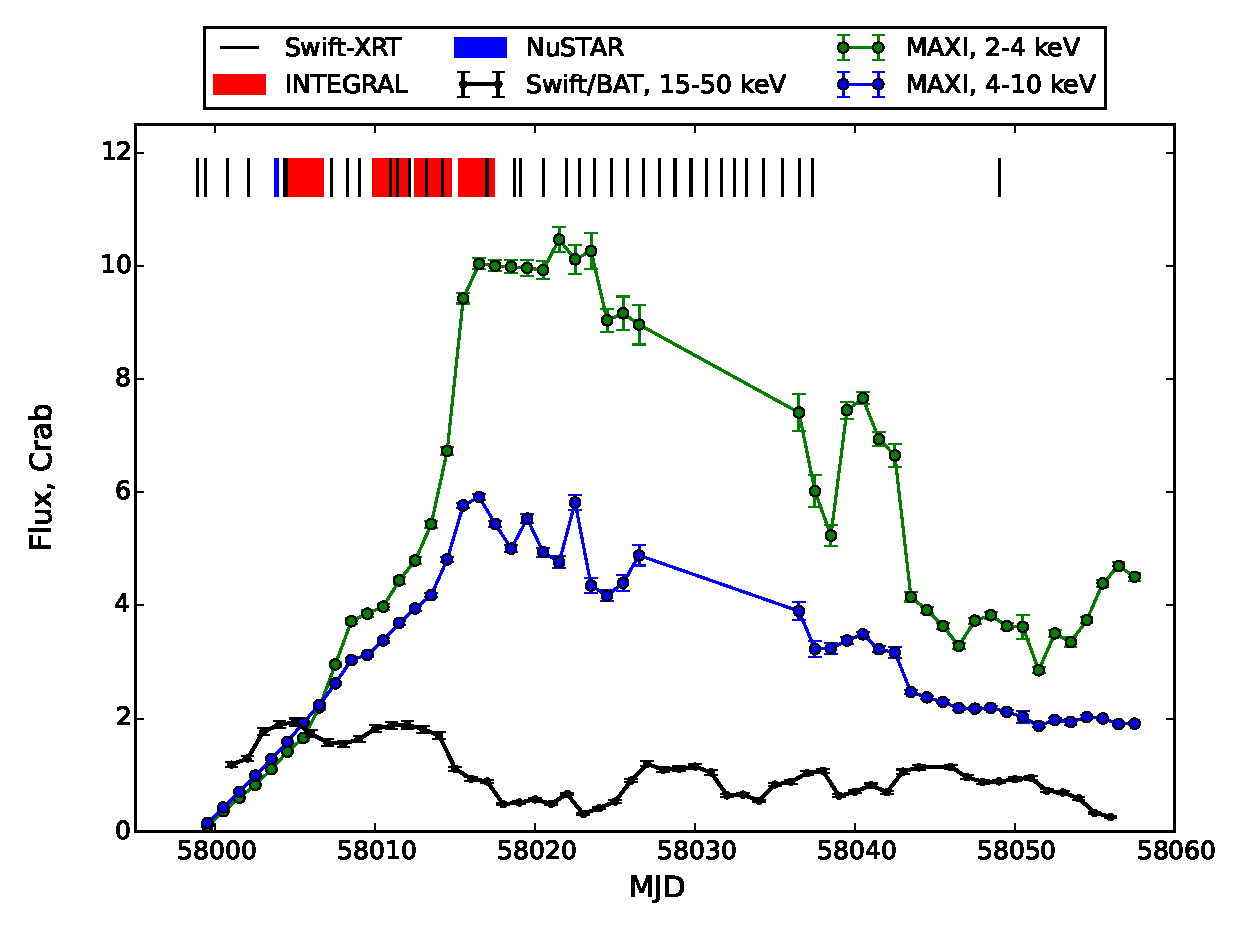
\includegraphics[scale=0.75]{overall_lc_v01.eps}}
\caption{Кривая блеска \maxi1535. Черными точками показан поток в диапазона 15--50 кэВ по данным \swiftb\,, зелеными и синими - данные \maxi в диапазонах 2--4 и 4--10 кэВ, соответственно. Красными линиями указаны наблюдения обсерватории \integral\,, черными и синими наблюдения телескопов \swiftx\, и \nustar. } 
\label{fig:lc}
\end{figure*} 


%----------------------------------------------------------------------------------------------


\acknowledgements

\label{lastpage}

%%%%%%%%%%%%%%%%%%%%%%%%%%%%%%%%%%%%%%%%%%%%%%%%%%%%%%%%%%%%%%%%%%%%%%%%%%%%%%%%%%

\bibliographystyle{pazh}
\bibliography{reflist_rus}
\end{document}
